\chapter{Parts rellevants de l'aplicació}

\section{Problema del repartiment de despeses}
Una de les funcions que ha de desenvolupar l'aplicació és fer una proposta sobre com solucionar els deutes existents entre els membres d'un grup. Tot i que en un principi es podria intentar resoldre pensant en les transaccions que ha fet cada membre, a l'hora de solucionar els deutes només cal tenir en compte el balanç de cada persona, tal com exposa David Vávra (creador de l'aplicació Settle Up) a la seva Tesis final de Màster (2012, p. 6-7) \cite{Settle_up}.

Un cop s'analitza el problema es pot veure que s'assembla al típic problema del transport, on s'ha de transportar de les fàbriques als magatzems, amb la diferència qualsevol emparellament té un cost nul i el que es busca és minimitzar el nombre de transaccions. 

Agafem com a exemple les següents persones amb els balanços de la taula \ref{table:balances}.

\begin{table}
\caption{Exemple dels balanços en un grup}
\label{table:balances}
\begin{tabular}{ | l | r |}
\hline
Persona & Balanç \\
\hline
Arnau & 20,33 \\
\hline
Berta & -3,90 \\
\hline
Càrol & -10,01 \\
\hline
David & 8,57 \\
\hline
Elena & -15,07 \\
\hline
\end{tabular}
\end{table}


\begin{table}
\caption{Exemple d'una resolució}
\label{table:resolution}
\begin{tabular}{ | r | l | r | r |}
 \hline
 & & 20,33 & 8,57 \\
 \hline
 & & Arnau & David \\
 \hline
 3,9 & Berta & & 3,9\\
 \hline
 10,01 & Càrol & 5,32 & 4,69\\
 \hline
 15,01 & Elena & 15,01 & \\
 \hline
\end{tabular}
\end{table}


Es pot veure que la Berta, la Càrol i l'Elena vindrien a ser les fàbriques i que l'Arnau i el David els magatzems als quals s'han d'enviar els diners. A la taula \ref{table:resolution} es mostra el problema juntament amb una solució possible.

Cal notar que degut a arrodoniments al calcular quan ha gastat cada persona en cada transacció es possible que la suma de tots els balanços no sigui 0. S'ha optat per beneficiar als creditors, de manera que tots els deutors paguin tot el que els correspon i que els creditors cobrin tot el que han deixat com a mínim, i si s'escau, alguns decimals de més.

David Vávra proposa solucionar el problema minimitzant només el nombre de transaccions total que s'hauran d'efectuar. Per a fer-ho proposa fer servir un mètode heurístic i posteriorment, si el nombre de persones del grup no es molt elevat, buscar la solució òptima. Per a trobar-la calcula totes les possibilitats. Aquesta manera de resoldre no és el més eficient possible. A més, si s'analitza en més profunditat el problema es pot veure que un bon repartiment no només ha de minimitzar el nombre total de transaccions. Entre altres aspectes que es poden tenir en compte, un bon repartiment serà aquell que:

\begin{itemize}
\item Minimitzi el nombre màxim de transaccions totals
\item Minimitzi el nombre màxim de transaccions que ha de fer una sola persona
\item Si es possible emparelli persones que es coneixen entre elles
\end{itemize}

Una manera de resoldre el problema tenint en compte aquests nous objectius és fent ús de la programació lineal. Concretament es té un de problema de \ac{PLEM}.
%TODO glossary

\subsection{Primera modelització del problema amb resolució exacte}
A continuació es modelarà el problema de solucionar els deutes d'un grup. Per a fer-ho només es buscara que minimitzi el nombre màxim de transaccions totals i el de transaccions que ha de fer una sola persona. Si bé, com ja s'ha dit, una bona solució també tindria en compte l'afinitat entre persones, això és més difícil de modelar i de descobrir sense forçar als usuaris a introduir molta informació. Tot i això la modelització serà prou flexible per a que si en un futur es vol afegir aquest objectiu, és pugui. 
\subsubsection{Dades}
\begin{description}
\item NC = nombre de creditors
\item ND = nombre de deutors
\item $D_{i}=$ diners que deu la persona \textbf{i} $\in (1 \ldots ND)$  [€].
\item $C_{j}=$ diners que li deuen a la persona \textbf{j} $\in (1 \ldots NC)$  [€].
\end{description}


\subsubsection{Variables}
\begin{description}
\item $x_{ij}=$ diners que dona la persona \textbf{i} $\in (1 \ldots ND)$ a la persona \textbf{j} $\in (1 \ldots NC)$  [€].
\item $p_{ij}=$ binaria que indica si la persona \textbf{i} $\in (1 \ldots ND)$ paga a la persona \textbf{j} $\in (1 \ldots NC)$.
\item a = màxim de transaccions dels deutors.
\item b = màxim de transaccions dels creditors
\end{description}

\subsubsection{Restriccions}
\begin{tabular}{l l}
$\sum\limits_{\forall j} x_{ij} \geq D_{i} \quad \forall i$ & Cada deutor ha de pagar com a mínim el que li correspon \\

$\sum\limits_{\forall i} x_{ij} \geq C_{j} \quad \forall j$ & Cada creditor ha de rebre com a mínim el que li correspon \\

$x_{ij} \leq M \cdot p_{ij} \quad \forall i \forall j$ & Forçar valor de $p_{ij}$ (M valor suficientment gran, per exemple $M=\sum\limits_{\forall i} D_{i} + \sum\limits_{\forall j} C_{j})$\\

$\sum\limits_{\forall j} p_{ij} \leq a \quad \forall i$ & Forçar valor de $a$ \\

$\sum\limits_{\forall i} p_{ij} \leq b \quad \forall j$ & Forçar valor de $b$ \\
\end{tabular}

\subsubsection{Funció Objectiu}
[min] $z = \sum\limits_{\forall i \forall j} p_{ij} + \lambda \cdot (a+b)$
Es busca minimitzar el nombre total de transaccions, així com el nombre de transaccions màximes que farà una sola persona
\subsubsection{Paràmetres}
$\lambda$ = usat per decidir el pes a la funció objectiu de cada part

\subsection{Modelització millorada amb resolució exacte}
La modelització anterior en alguns casos no trobava una solució factible, degut als arrodoniments a l'hora de calcular els balanços (pas previ a la solució del \ac{PLEM}).
La idea general d'aquesta modelització es calcular els diners que un deutor pagà a un creditor que formen part del deute per una banda i per l'altre els diners extra que ha de pagar (tot i que no li corresponen). Aquests diners extra sortiran a la funció objectiu amb una penalització molt elevada per tal que al resoldre el \ac{PLEM} només siguin més grans de zero en cas de ser necessari. Vist per la banda dels creditors es farà el mateix, es calcularà els diners extra que han de rebre per tal que els deutors paguin el necessari. De fet aquestes dues variables corresponen a les variables de marge associades a la primera i segona restricció respectivament.

\subsubsection{Dades}
\begin{description}
\item $x_{ij}=$ diners que dona la persona \textbf{i} $\in (1 \ldots ND)$ a la persona \textbf{j} $\in (1 \ldots NC)$  [€].
\item $p_{ij}=$ binaria que indica si la persona \textbf{i} $\in (1 \ldots ND)$ paga a la persona \textbf{j} $\in (1 \ldots NC)$.
\item a = màxim de transaccions dels deutors.
\item b = màxim de transaccions dels creditors
\end{description}

\subsubsection{Variables}
\begin{description}
\item $x_{ij}=$ diners que dona la persona \textbf{i} $\in (1 \ldots ND)$ a la persona \textbf{j} $\in (1 \ldots NC)$  [€].
\item $p_{ij}=$ binaria que indica si la persona \textbf{i} $\in (1 \ldots ND)$ paga a la persona \textbf{j} $\in (1 \ldots NC)$.
\item a = màxim de transaccions dels deutors.
\item b = màxim de transaccions dels creditors 
\item $t_{i}=$ diners extres que ha de pagar la persona \textbf{i} $\in (1 \ldots ND)$  [€].
\item $q_{j}=$ diners extres que ha de rebre la persona \textbf{j} $\in (1 \ldots NC)$  [€].
\end{description}

\subsubsection{Restriccions}
\begin{tabular}{l l}
$\sum\limits_{\forall j} x_{ij} + t_{i} = D_{i} \quad \forall i$ & Cada deutor ha de pagar com a mínim el que li correspon \\

$\sum\limits_{\forall i} x_{ij} + q_{j} = C_{j} \quad \forall j$ & Cada creditor ha de rebre com a mínim el que li correspon \\

$x_{ij} \leq M \cdot p_{ij} \quad \forall i \forall j$ & Forçar valor de $p_{ij}$ (M valor suficientment gran, per exemple $M=\sum\limits_{\forall i} D_{i} + \sum\limits_{\forall j} C_{j})$\\

$\sum\limits_{\forall j} p_{ij} \leq a \quad \forall i$ & Forçar valor de $a$ \\

$\sum\limits_{\forall i} p_{ij} \leq b \quad \forall j$ & Forçar valor de $b$ \\
\end{tabular}

\subsubsection{Funció Objectiu}
[min] $z = \sum\limits_{\forall i \forall j} p_{ij} + \lambda_{1} \cdot \sum\limits_{\forall i} t_{i} + \lambda_{2} \cdot \sum\limits_{\forall j} q_{j} + \lambda_{3} \cdot a + \lambda_{4} \cdot b $

Es busca minimitzar el nombre total de transaccions, així com el nombre de transaccions màximes que farà una sola persona
\subsubsection{Paràmetres}
$\lambda$ = usat per decidir el pes a la funció objectiu de cada part

\subsubsection{Post-procés}
Finalment, per calcular que ha de pagar cada persona es repartiran els diners extres que han de rebre els creditors per tal que tots ells rebin com a mínim tot el que es deu. No es repartiran els diners extres que han de pagar els deutors ja que amb què els creditors rebin el que se'ls hi devia ja n'hi ha prou. Aquests diners extres que un creditor ha de rebre es repartiran entre totes les persones que han de donar-li diners, deixant de banda els deutors que no han de pagar res a aquell creditor. 

Per tant el deutor \textbf{i} pagarà al creditor \textbf{j}: $\frac{x_{ij} + q_{j}*p_{ij}}{\sum\limits_{\forall k} p_{ik}}$

\subsection{Estudi del temps computacional de la modelització millorada}
Un cop es té una bona modelització del problema, cal provar-la amb un aparell i dades reals per comprovar que el temps necessari per resoldre el problema no sigui excessiu. Per a fer-ho s'ha utilitzat un \gls{Nexus_5} i la llibreria per a resoldre problemes de programació lineal \gls{lp_solve}.

En un primer moment s'ha fet servir les dades de 17 balanços provinent de grups de despeses reals creats amb l'aplicació Settle Up. S'ha calculat el temps de resolució per a cada cas 5 cops i s'ha fet la mitjana per cada cas. Analitzant les dades en un primer moment (figura \ref{fig:PLEM_1}) sembla que:

\begin{enumerate}
\item El temps d'execució és sempre molt baix
\item El temps depèn de forma logarítmica del nombre de nodes (N) del problema. ($N = 2*NC*ND + NC + ND + 2$)
\end{enumerate}

\begin{figure}[ht]
\centering
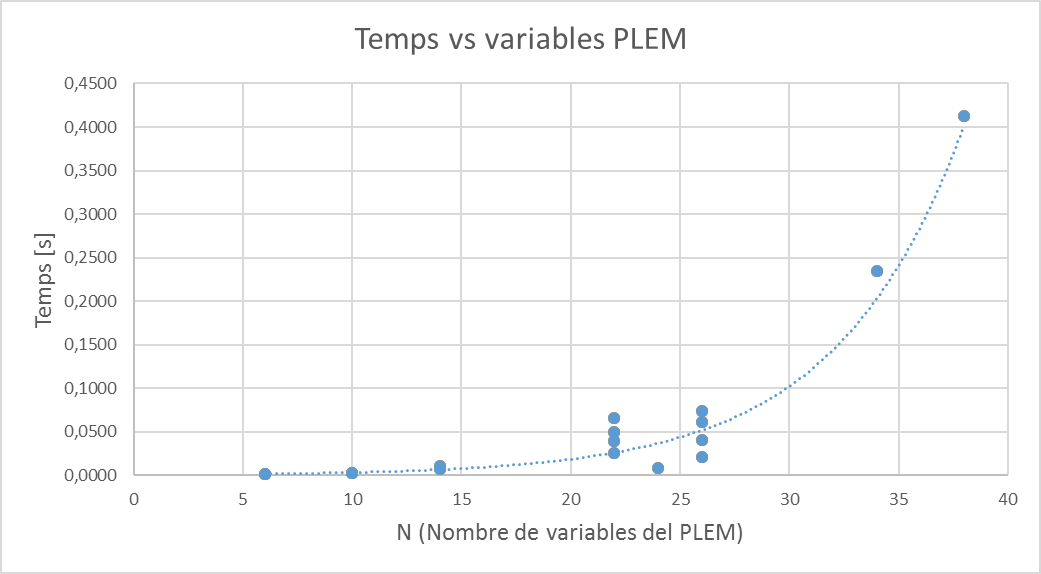
\includegraphics[scale=0.8]{PLEM_temps_2.png}
\caption{Temps per resoldre el PLEM en funció del nombre de nodes (N)}\label{fig:PLEM_1}
\end{figure}

Per a comprovar aquestes hipòtesis s'ha afegit un joc de dades inventat on el nombre de nodes fos més elevat. Amb aquest joc de dades el temps ja no era menor d'un segon (figura \ref{fig:PLEM_2}), com en els altres casos, sinó que estava prop dels 3 minuts. 

\begin{figure}[ht]
\centering
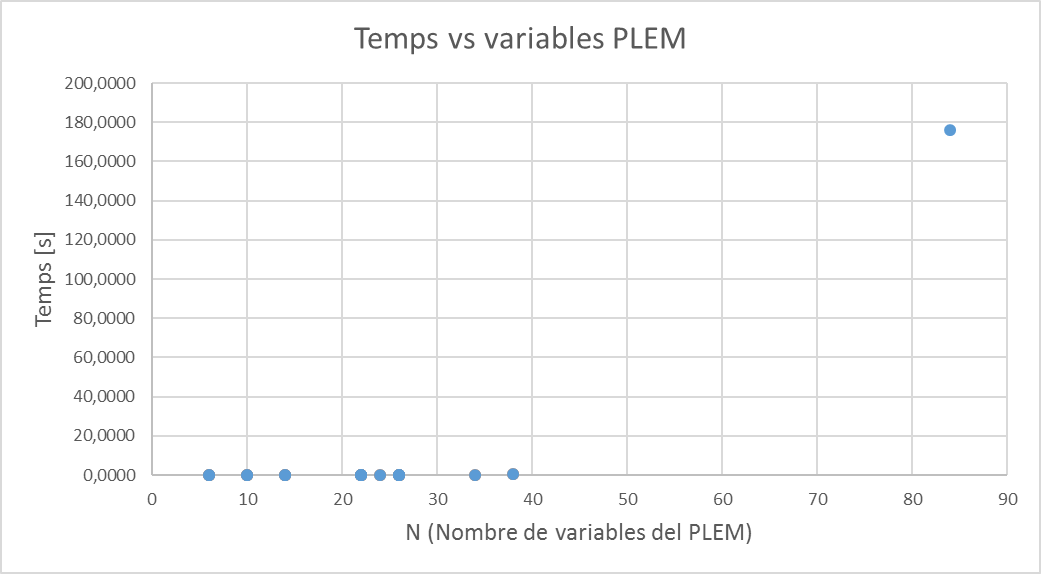
\includegraphics[scale=0.8]{PLEM_temps_1.png}
\caption{Temps per resoldre el PLEM en funció del nombre de nodes (N)}\label{fig:PLEM_2}
\end{figure}

Finalment i després de diverses proves s'ha comprovat que el temps en realitat depèn de forma logarítmica del nombre de deutors i creditors conjuntament, tal com es pot veure a la figura \ref{fig:PLEM_3}. S'han emprat 61 jocs de dades creats de manera que es calculessin la majoria de combinacions possibles de NC i ND amb un temps d'execució relativament baix. Com abans, cada cas s'ha calculat 5 cops i s'ha fet la mitjana dels 5 temps.

%TODO citar les dades

\begin{figure}[ht]
\centering
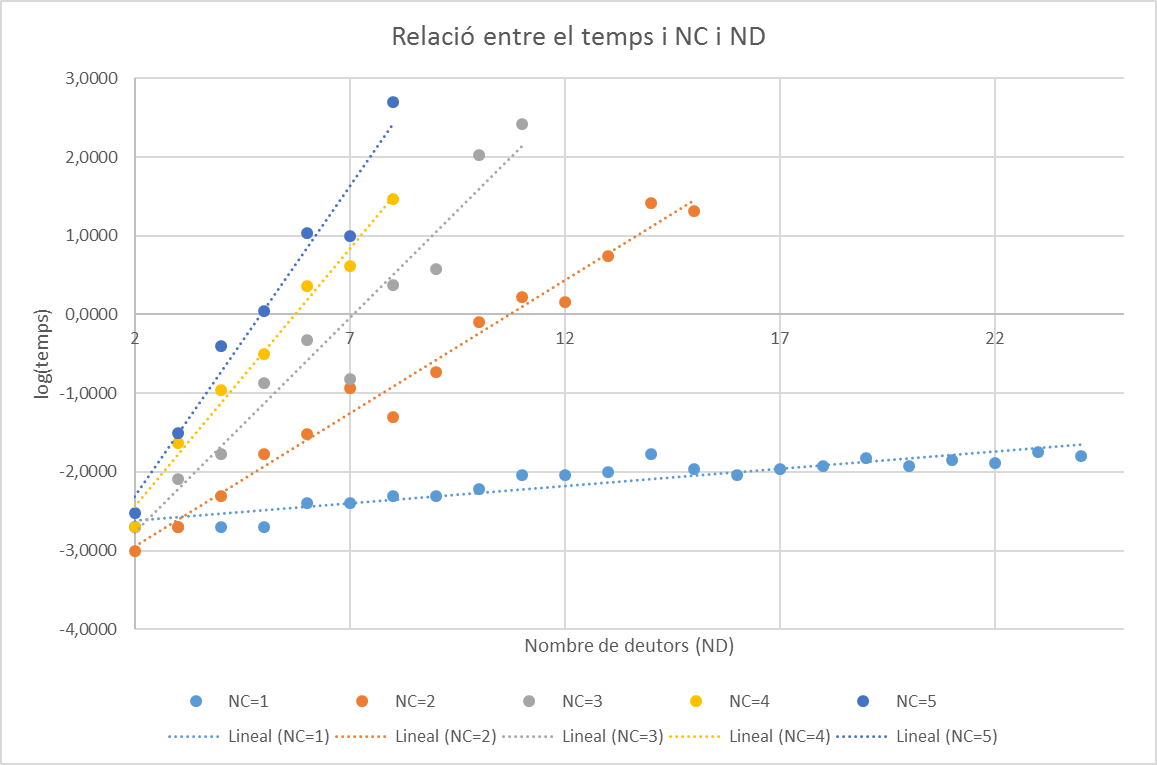
\includegraphics[scale=0.8]{PLEM_temps_3.png}
\caption{Temps per resoldre el PLEM en funció del nombre de creditors (NC) i dels deutors (ND)}\label{fig:PLEM_3}
\end{figure}

Aquest temps d'execució elevat és degut al \gls{BB}. Per trobar una solució amb valors reals, el temps és menor d'un segon, però al intentar trobar una solució amb valors enters tot assegurant què és òptima el temps ja es elevat.

\subsection{Algoritme final}
Finalment s'ha decidit calcular la solució òptima, restringint el programa a un temps d'execució de 3 segons, juntament amb una la resolució heurística que proposa David Vávra (2012, p. 6-7) \cite{Settle_up}. Si en aquest temps el programa troba una solució factible, és compararà amb la solució heurística per veure quin té millor valor de la funció objectiu. Si amb la resolució òptima no s'arriba a una solució factible s'utilitzarà l'aconseguida amb l'heurística. 

\section{Disseny de la base de dades}
A l'hora d'emmagatzemar les dades de la aplicació s'ha optat per fer servir \gls{SQLite} de forma local al \gls{smartphone} i fer ús del \gls{BAAS} Parse.com. Per tant s'ha dissenyat una base de dades local i una altre al núvol. La base de dades principal és la local i la del núvol està com a còpia de seguretat i per garantir la sincronització multidispositiu. Les taules que han de ser llegides per varies persones s'han partir en dues, una privada i una pública, al emmagatzemar-les al núvol de manera que el mínim d'informació és accessible per als usuaris que no l'han creat.

A la figura \ref{fig:db_sqlite} es pot veure el disseny de la base de dades local, a la figura \ref{fig:db_parse} es pot veure la base de dades al núvol i a la figura \ref{fig:db_private_shared} és pot veure quines columnes són privades i quines públiques a cada taula. 

\begin{figure}[ht]
\centering
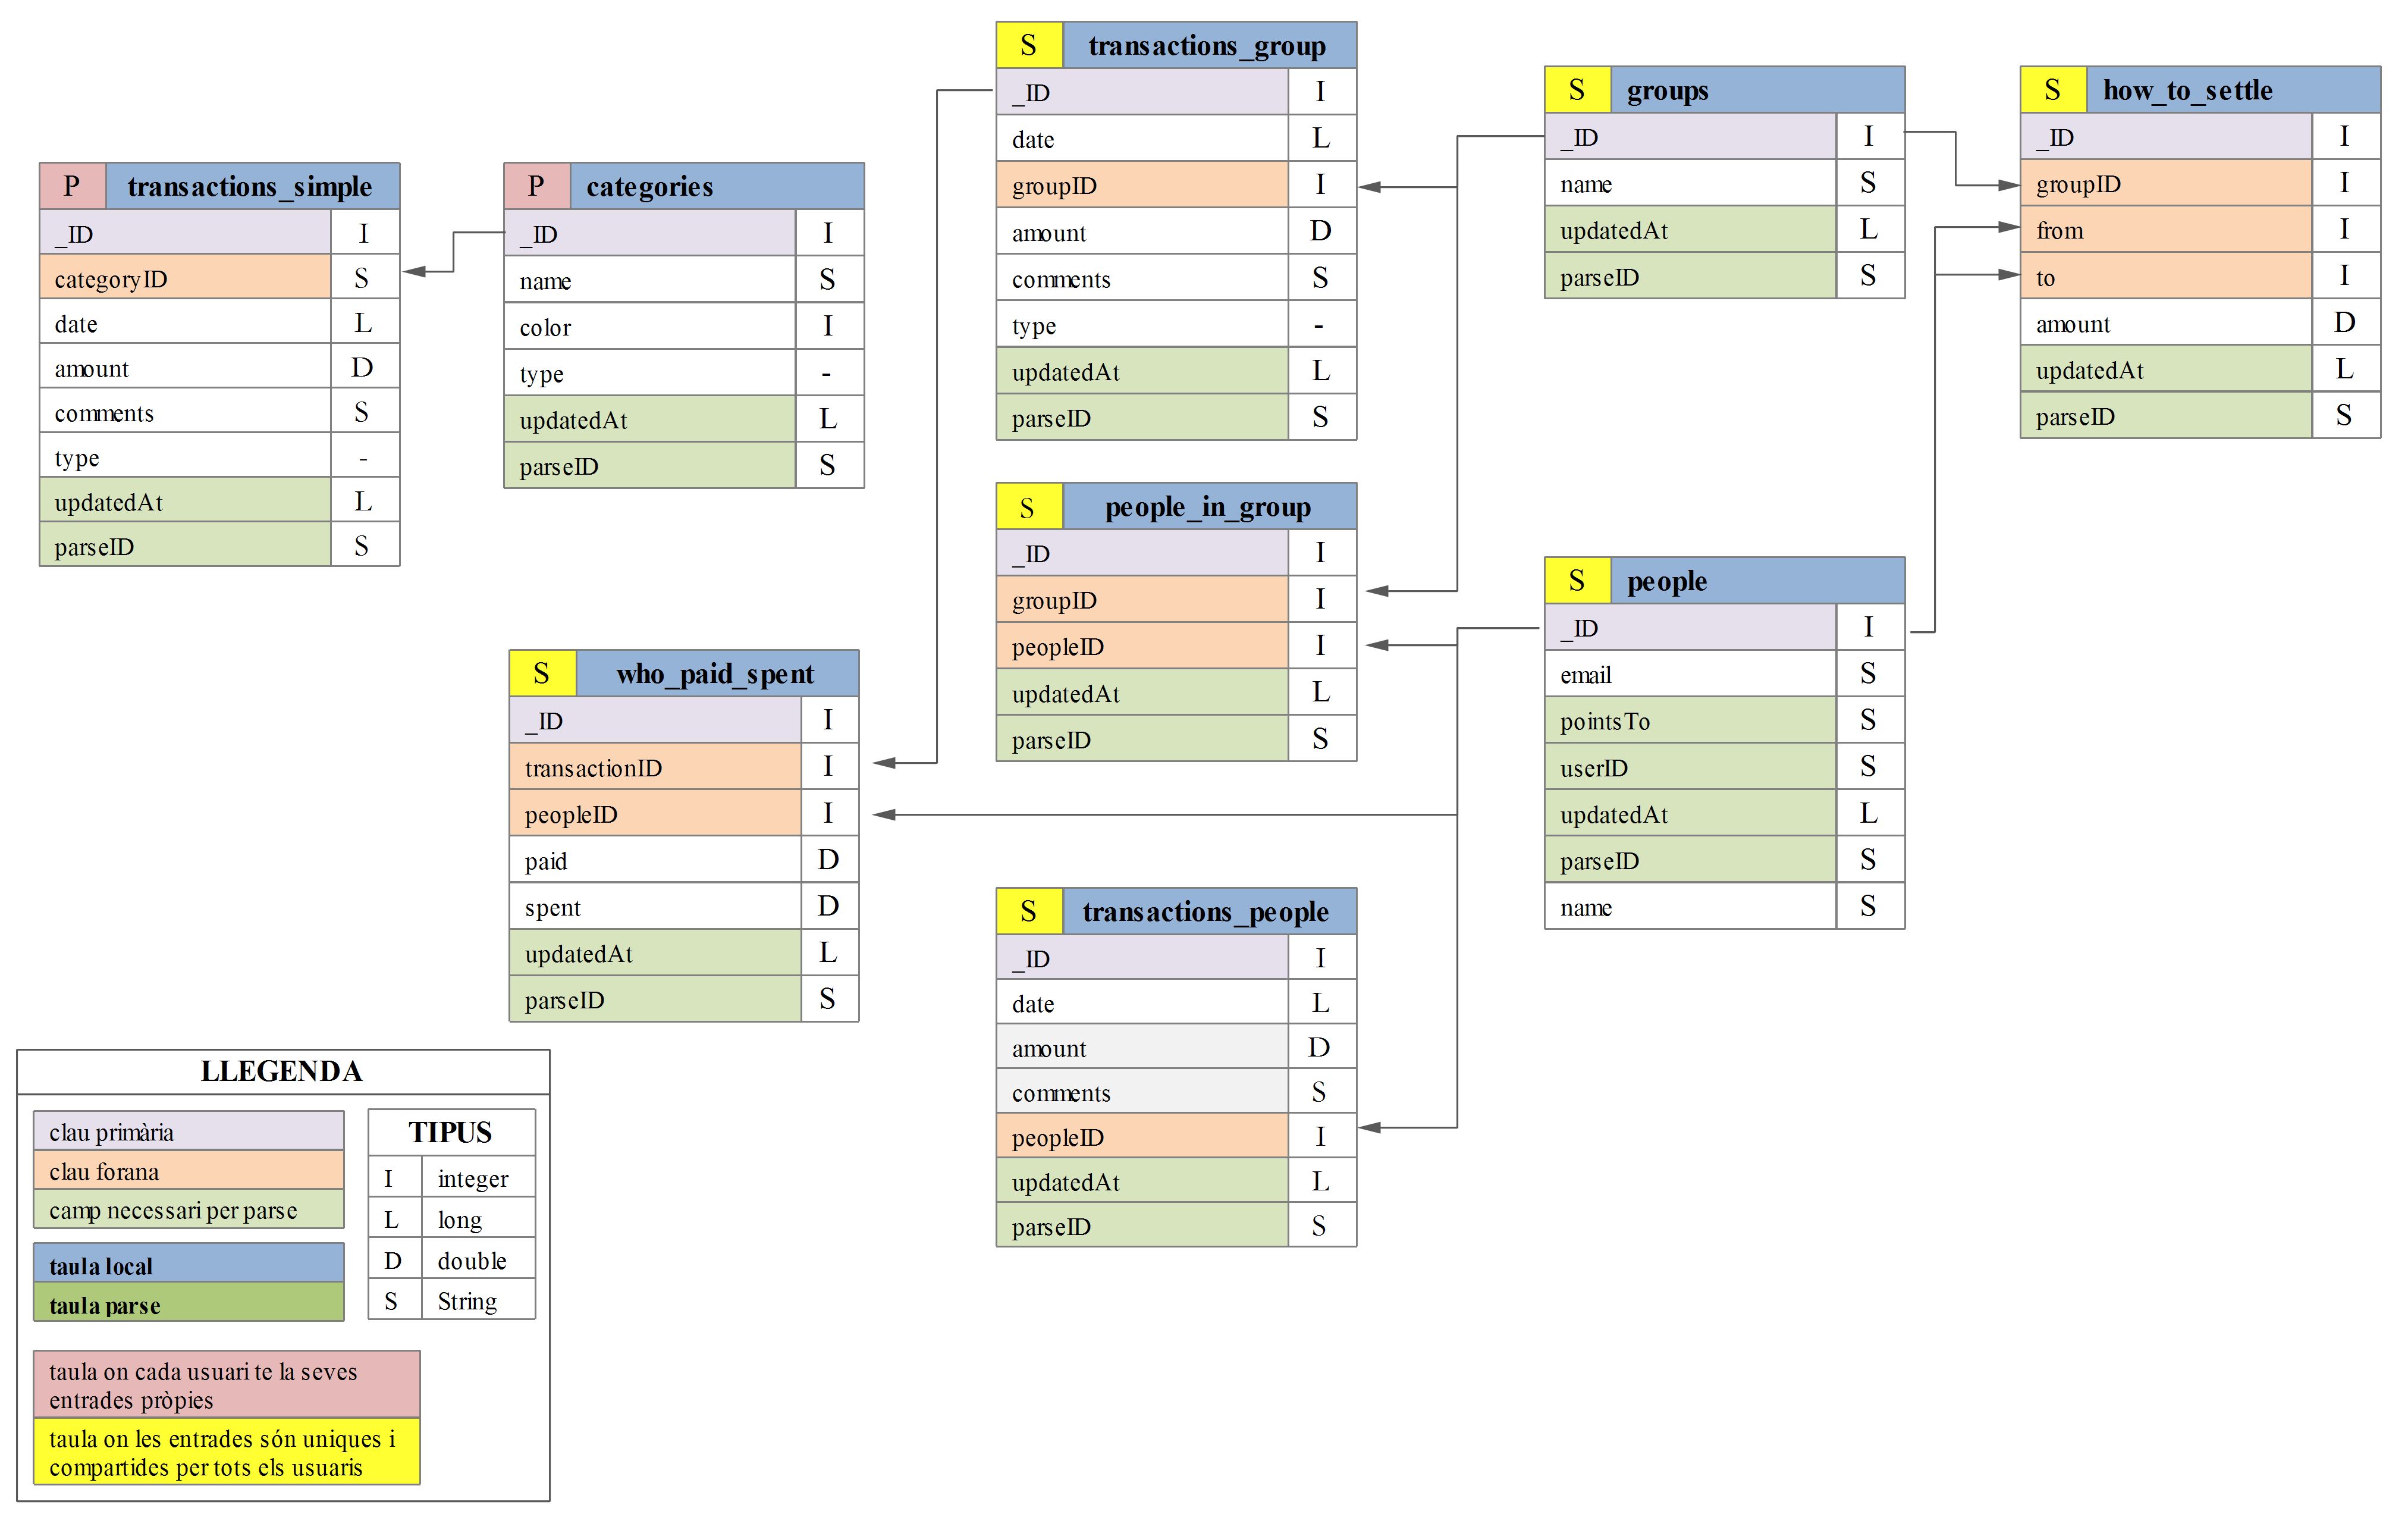
\includegraphics[scale=0.44]{db_sqlite.png}
\caption{Base de dades local amb SQLite}\label{fig:db_sqlite}
\end{figure}

\begin{figure}[ht]
\centering
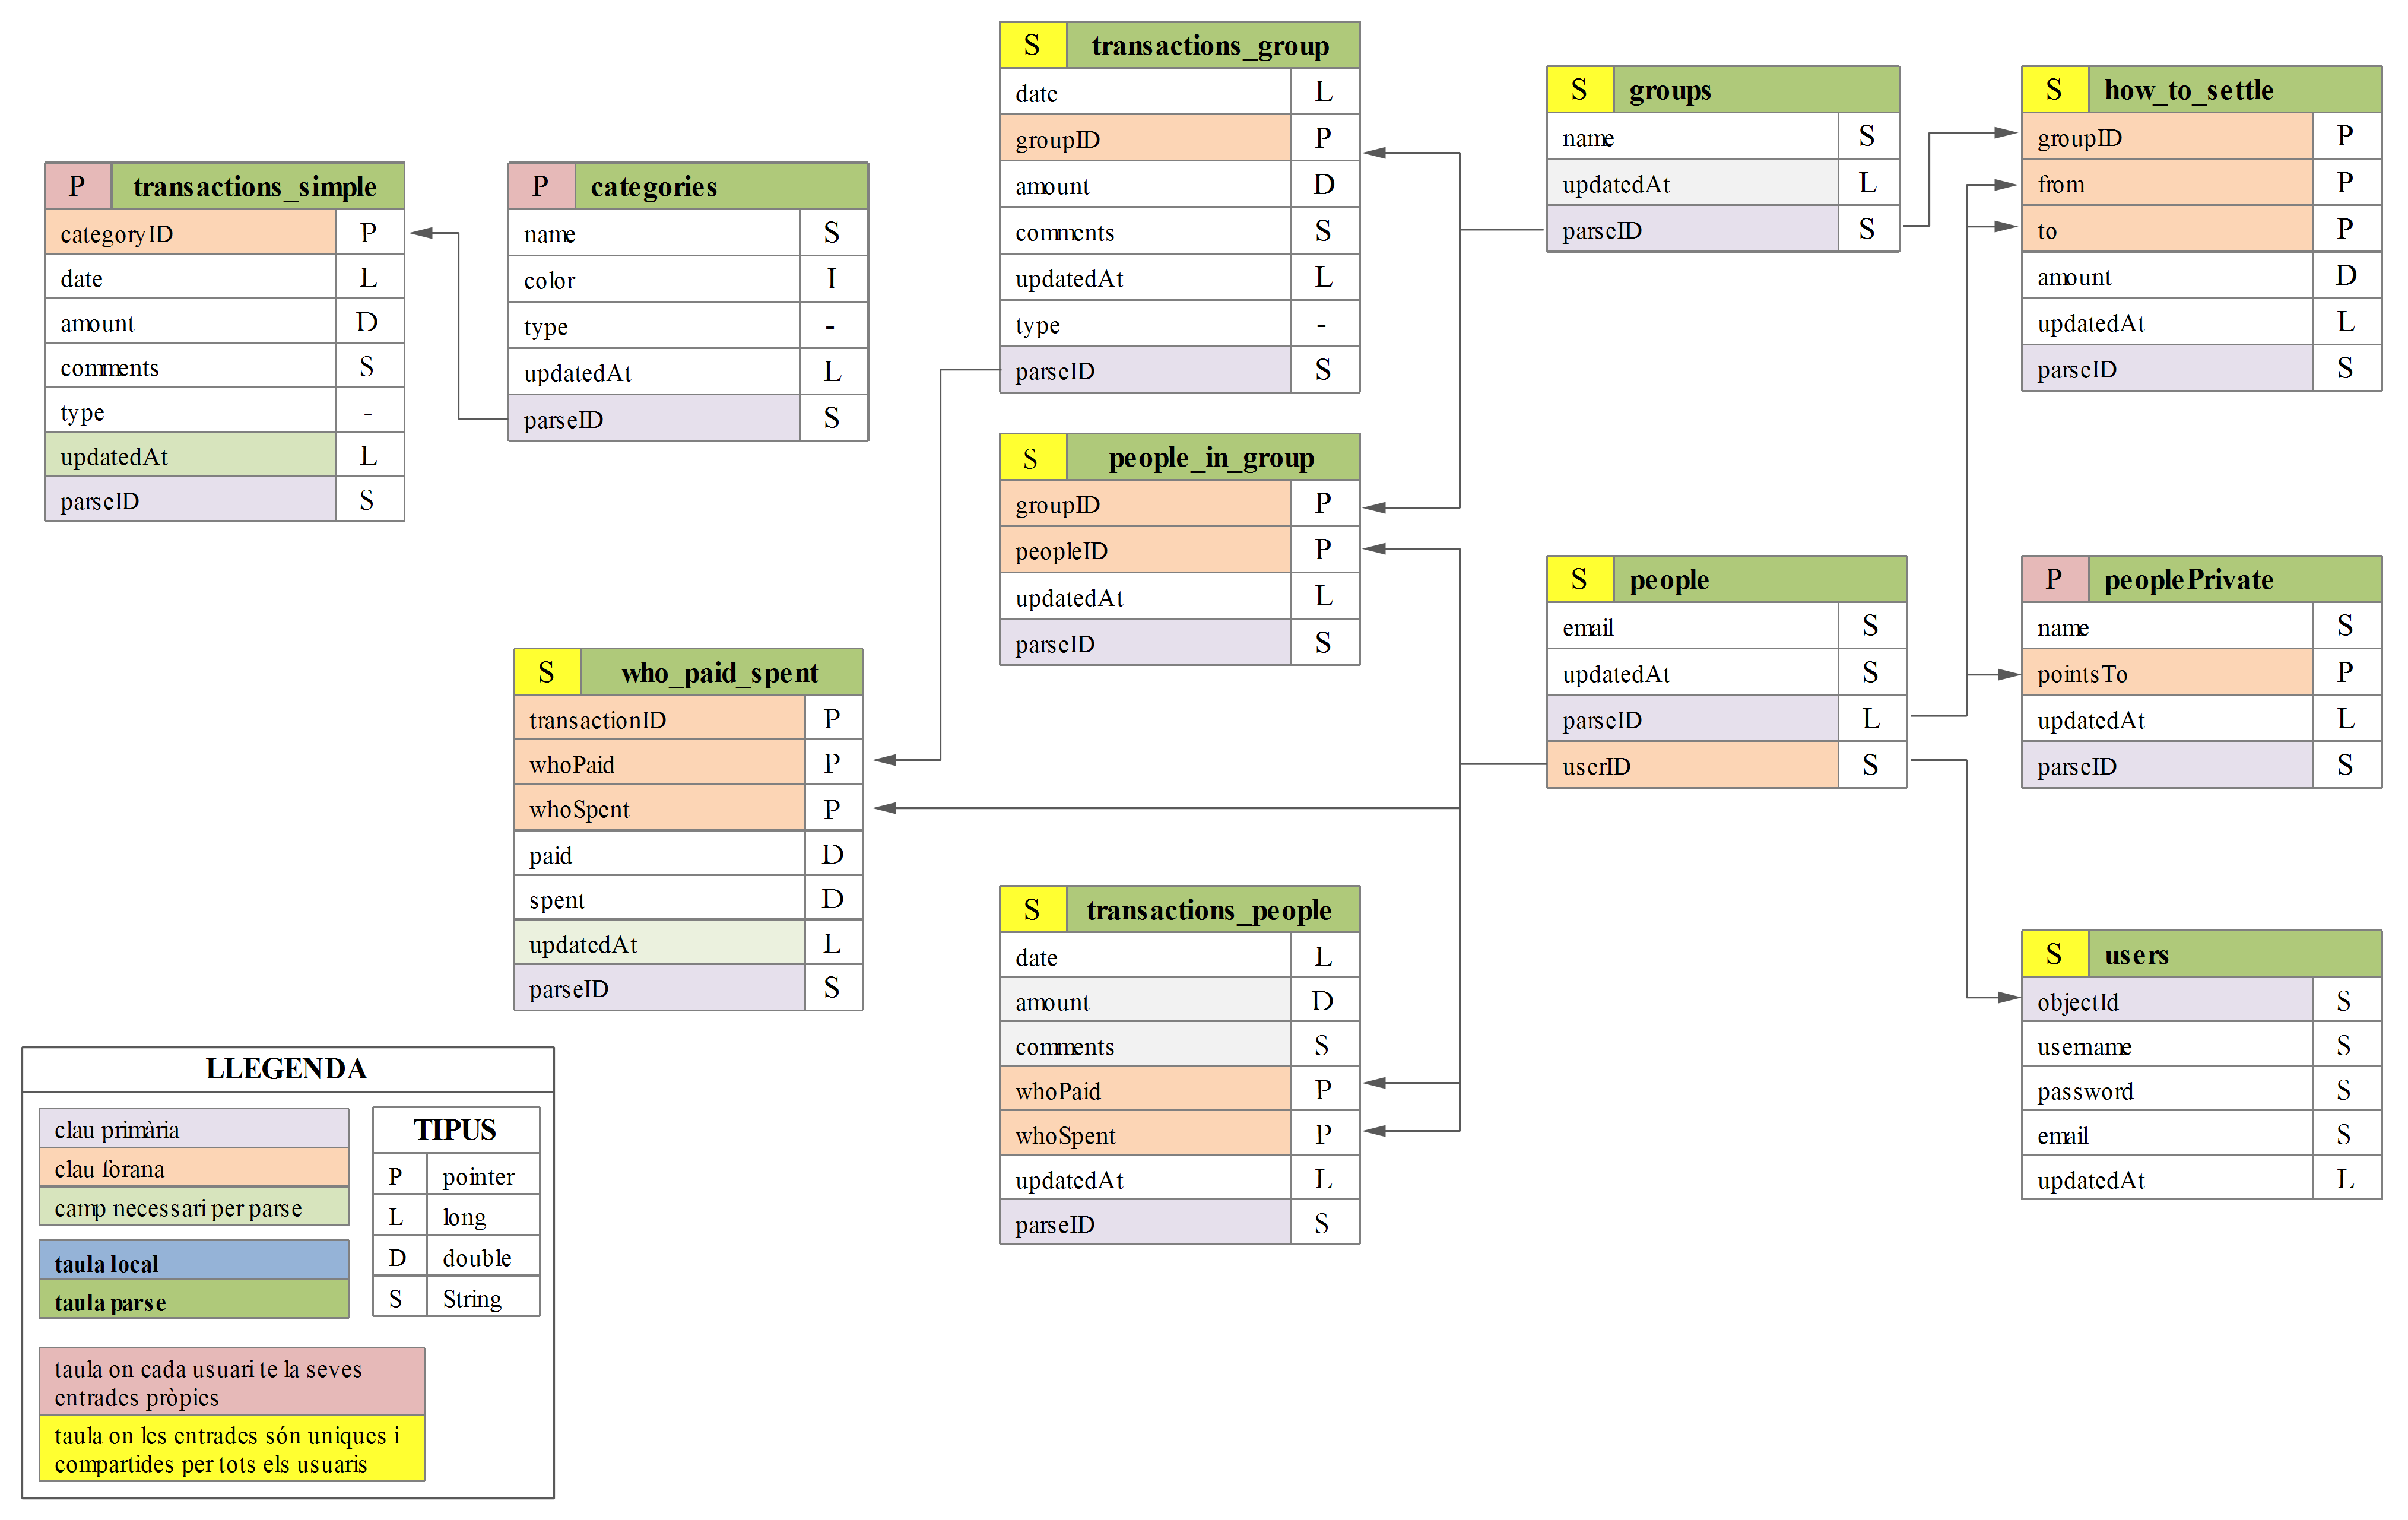
\includegraphics[scale=0.44]{db_parse.png}
\caption{Base de dades al núvol amb Parse.com}\label{fig:db_parse}
\end{figure}

\begin{figure}[ht]
\centering
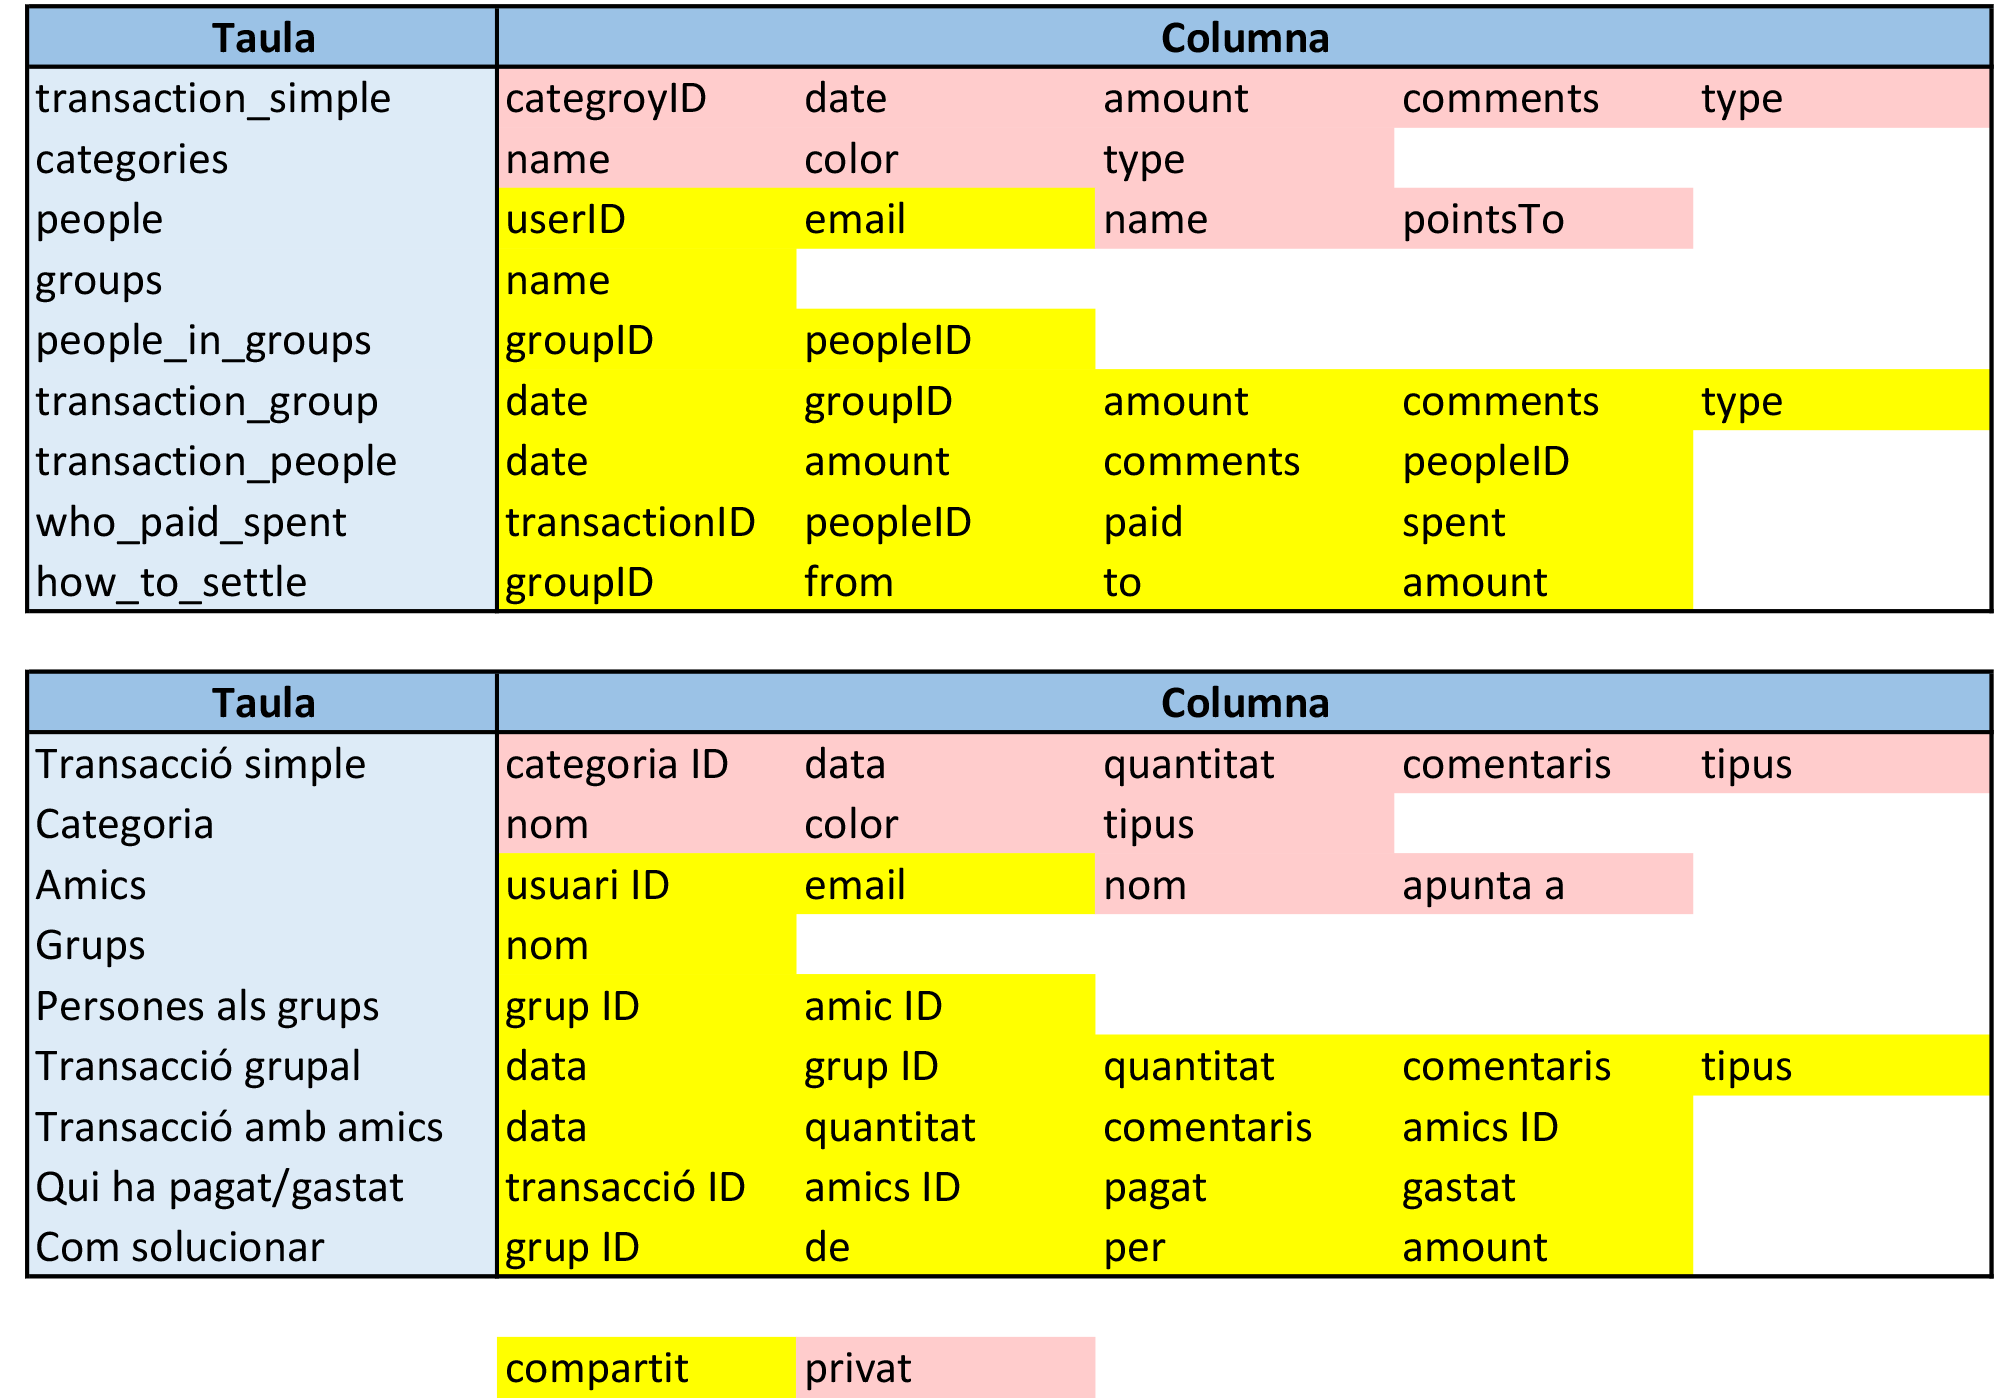
\includegraphics[scale=0.8]{db_private_shared.png}
\caption{Columnes privades i compartides de cada taula}\label{fig:db_private_shared}
\end{figure}
